%%% Exemplo de utilização da classe ITA
%%%
%%%   por        Fábio Fagundes Silveira   -  ffs [at] ita [dot] br
%%%              Benedito C. O. Maciel     -  bcmaciel [at] ita [dot] br
%%%              Giovani Volnei Meinertz   -  giovani [at] ita [dot] br
%%%    	         Hudson Alberto Bode       -  bode [at] ita [dot]br
%%%    	         P. I. Braga de Queiroz    -  pi [at] ita [dot] br
%%%    	         Jorge A. B. Gripp         -  gripp [at] ita [dot] br
%%%    	         Juliano Monte-Mor         -  jamontemor [at] yahoo [dot] com [dot] br
%%%    	         Tarcisio A. B. Gripp      -  tarcisio.gripp [at] gmail [dot] com
%%%
%%%   Versão para overleaf:
%%%   por        Alejandro A. Rios Cruz    - aarc.88@gmail.com
%%%              Saulo Gómez               - sagomezs@unal.edu.co
%%%              Ocimar Santos             - ocimar.acad@gmail.com
%%%
%%%   Template disponibilizado em:
%%%              Overleaf: https://pt.overleaf.com/latex/templates/thesis-template-aeronautics-institute-of-technology-ita/yhfrqqydpygk
%%%
%%%   Contribuia você também!
%%%              GitHub:   https://github.com/gabriellnuness/Template_Thesis_ITA
%%%
%%%  IMPORTANTE: O texto contido neste exemplo nao significa absolutamente nada.  :-)
%%%              O intuito aqui eh demonstrar os comandos criados na classe e suas
%%%              respectivas utilizacoes.
%%%
%%%  Tese.tex  2016-08-25
%%%  $HeadURL: http://www.apgita.org.br/apgita/teses-e-latex.php $
%%%
%%% ITALUS
%%% Instituto Tecnológico de Aeronáutica --- ITA, Sao Jose dos Campos, Brasil
%%%                   http://groups.yahoo.com/group/italus/
%%% Discussion list: italus {at} yahoogroups.com
%%%
%++++++++++++++++++++++++++++++++++++++++++++++++++++++++++++++++++++++++++++++
% Para alterar o TIPO DE DOCUMENTO, preencher a linha abaixo \documentclass[?]{?}
%   \documentclass[tg]{ita}			= Trabalho de Graduacao
%   \documentclass[tgfem]{ita}	= Para Engenheiras
%   								msc     		= Dissertacao de Mestrado
%   								mscfem   		= Para Mestras
%   								dsc      		= Tese de Doutorado
%   								dscfem   		= Para Doutoras
%   								quali    		= Exame de Qualificacao
%   								qualifem 		= Exame de Qualificacao para Doutoras
% Para 'Draft Version'/'Versao Preliminar' com data no rodape, adicionar 'dv':
%   \documentclass[dsc, dv]{ita}
% Para trabalhos em Inglês, adicionar 'eng':
%   \documentclass[dsc, eng]{ita}
%		\documentclass[dsc, eng, dv]{ita}
%++++++++++++++++++++++++++++++++++++++++++++++++++++++++++++++++++++++++++++++
\documentclass[dsc]{ita}    % ITA.cls based on standard book.cls
% Quando alterar a classe, por exemplo de [msc] para [msc, eng]) rode mais uma vez o botão BUILD OUTPUT caso haja erro
\usepackage{ae}
\usepackage{graphicx}
\usepackage{epsfig}
\usepackage{amsmath}
\usepackage{amssymb}
\usepackage{subfig}
\usepackage{multirow}
\usepackage{float}
\usepackage{amsthm}
\usepackage{url}         % formats URL addresses properly
\usepackage{appendix}    % allows appendix section to be included
\usepackage{lscape}      % allows a page to be rendered in landscape mode
\usepackage{multicol}    % allows text in multi columns
\usepackage{cancel}      % needed to show canceled terms in equations
\usepackage{lettrine}
\usepackage{float}
\usepackage{placeins}


%HHHHHHHHHHHHHHHHHHHHHHHHHHHHHHHHHHHHHHHHHHHHHHHHHHHHHHHHHHHHHHHHHHHHHHHHHHHHHHHHHHHHHHHHHHHHHHHHHHHHHHHHHHHH
\addbibresource{Referencias/referencias.bib}

%HHHHHHHHHHHHHHHHHHHHHHHHHHHHHHHHHHHHHHHHHHHHHHHHHHHHHHHHHHHHHHHHHHHHHHHHHHHHHHHHHHHHHHHHHHHHHHHHHHHHHHHHHHHH
%\usepackage{subfigure}
%\usepackage{subfigmat}
%PACOTEFIGURAS_SE _ERRADO_ESXCLUIR_ACIMA
\usepackage{booktabs}
%PACOTETABELAS_SE _ERRADO_ESXCLUIR_ACIMA
%HHHHHHHHHHHHHHHHHHHHHHHHHHHHHHHHHHHHHHHHHHHHHHHHHHHHHHHHHHHHHHHHHHHHHHHHHHHHHHHHHHHHHHHHHHHHHHHHHHHHHHHHHHHH

%++++++++++++++++++++++++++++++++++++++++++++++++++++++++++++++++++++++++++++++
% Espaçamento padrão de todo o documento
%++++++++++++++++++++++++++++++++++++++++++++++++++++++++++++++++++++++++++++++
\onehalfspacing

%singlespacing Para um espaçamento simples
%onehalfspacing Para um espaçamento de 1,5
%doublespacing Para um espaçamento duplo

%++++++++++++++++++++++++++++++++++++++++++++++++++++++++++++++++++++++++++++++
% Identificacoes (se o trabalho for em inglês, insira os dados em inglês)
% Para entradas abreviadas de Professora (Profa.) em português escreva: Prof$^\textnormal{a}$.
%++++++++++++++++++++++++++++++++++++++++++++++++++++++++++++++++++++++++++++++
\course{Aerospace Engineering}  % Programa de PG ou Curso de Graduação
%\area{Aircraft Design} % Área de concentração na PG (Não utilizado no caso de TG)

% Autor do trabalho: Nome Sobrenome
\authorgender{masc}                     %sexo: masc ou fem
\author{Pedro Kuntz}{Puglia}
\itaauthoraddress{Rua H8X, Ap. XXX}{12.228-46?}{São José dos Campos--SP}

% Titulo da Tese/Dissertação
\title{Orbital Maneuver Optimization}

% Orientador
\advisorgender{masc}                    % masc ou fem
\advisor{Prof.~Dr.}{Willer Gomes dos Santos}{ITA}

% Coorientador (Caso não haja coorientador, colocar ambas as variáveis \coadvisorgender e \coadvisor comentadas, com um % na frente)
\coadvisorgender{masc}									% masc ou fem
\coadvisor{Prof.}{Emilien Flayac}{ISAE-SUPAERO}

% Pró-reitor da Pós-graduação
\bossgender{masc}												% masc ou fem
\boss{Prof.~Dr.}{John von Neumann}

%Coordenador do curso no caso de TG
\bosscoursegender{masc}									% masc ou fem
\bosscourse{Prof.~Dr.}{John Walker}

% Palavras-Chaves informadas pela Biblioteca -> utilizada na CIP
\kwcip{Optimization}
\kwcip{control}
\kwcip{orbital mechanics}

% membros da banca examinadora

\examiner{Prof. Dr.}{Alan Turing}{Presidente}{ITA}
\examiner{Prof. Dr.}{Linus Torwald}{}{UXXX}
\examiner{Prof. Dr.}{Richard Stallman}{}{UYYY}
\examiner{Prof. Dr.}{Donald Duck}{}{DYSNEY}
\examiner{Prof. Dr.}{Mickey Mouse}{}{DISNEY}

% Data da defesa (mês em maiúsculo, se trabalho em inglês, e minúsculo se trabalho em português)
\date{23}{novembro}{2022}

% Número CDU - (somente para TG)
\cdu{???.??}

% Glossario
\makenoidxglossaries % to use glossaries pkg
\frontmatter


\begin{longtable}{ll}
LEO & Low Earth Orbit \\
RAAN & Right ascension of the ascending node \\
TPBVP & Two Point Boundary Value Problem \\
STM & State Transition Matrix \\
PVTM & Primer Vector Transition Matrix \\
PVDE & Primer Vector Differential Equation \\
\end{longtable}


\begin{longtable}{ll}
\(\mathbf{F}\) & Empuxo propulsivo \\
\(\dot{m}\) & Vazão mássica \\
\(v_e\) & Velocidade de exaustão média \\
\(p_c\) & Pressão de câmara \\
\(p_e\) & Pressão de saída média \\
\(p_{amb}\) & Pressão ambiente \\
\(A_c\) & Área da seção transversal da câmara \\
\(A_e\) & Área da seção transversal da saída da tubeira \\
\(A_t\) & Área da seção transversal da garganta \\
\(\varepsilon \) & Razão de expansão \\
\(I_{\mathrm{sp}}\) & Impulso específico \\
\(C_F\) & Coeficiente de empuxo \\
\(C^*\) & Velocidade característica \\
\(F_x\) & Força horizontal, transversal ao motor foguete \\
\(F_y\) & Força vertical, na direção do empuxo propulsivo \\
\(M\) & Torque resultante \\
\(\delta \) & Deflexão da lâmina (\textit{jet vane}) \\
\(F_{x\delta}\) & Derivada da força lateral em relação à deflexão da lâmina \\
\(M_\delta \) & Derivada de momento em relação à deflexão da lâmina
\end{longtable}



\begin{document}
% Folha de Rosto e Capa para o caso do TG
\maketitle

% Dedicatoria: Nao esqueca essa secao  ... :-)
\begin{itadedication}
Aos amigos da Graduação e Pós-Graduação do ITA por motivarem tanto a criação deste template pelo Fábio Fagundes Silveira quanto por motivarem a mim e outras pessoas a atualizarem e aprimorarem este excelente trabalho.
\end{itadedication}

% Agradecimentos
\begin{itathanks}
Agradeço ao professor Leonardo Gouvêa por, certo dia falando sobre qualquer coisa, levantar a possibilidade deste trabalho, e por auxiliar no que é necessário auxílio e dar liberdade no que é necessário liberdade.

Agradeço também ao João Vitor Baldo e Arthur Zoppi, que acompanharam todas as minhas impressões 3D no Laboratório Aberto do CCM-ITA, sempre dando dicas e sugestões que iam além do esperado deles. Obrigado por transformar impressões problemáticas e fracassadas em momentos de descontração e aprendizado sobre mundo real.

Agradeço por fim a toda a equipe do Laboratório Feng, que foi recrutada por acaso no meio do caminho para minha iniciação científica. Agradeço ao Prof. Dr. Tiago Barbosa, que permitiu o uso do laboratório, e ao professor André Fernando de Castro, que certo dia por acaso resolveu (quase) todos os problemas experimentais do meu trabalho comigo. Agradeço especialmente aos técnicos Newton, que me auxiliou com toda a montagem mecânica do experimento, e Wilson, que me acompanhou pelas várias horas de montagem e calibração.

Por fim agradeço à minha família, que sempre me incentivou, e aos meus amigos de ITA e H8, que inúmeras vezes me ouviram falar detalhadamente sobre os problemas deste trabalho.
\end{itathanks}

% Epígrafe
\thispagestyle{empty}
\ifhyperref\pdfbookmark[0]{\nameepigraphe}{epigrafe}\fi
\begin{flushright}
\begin{spacing}{1}
\mbox{}\vfill
{\sffamily\itshape
``If I have seen farther than others,\\
it is because I stood on the shoulders of giants.''\\}
--- \textsc{Sir~Isaac Newton}

\end{spacing}
\end{flushright}

% Resumo
\begin{abstract}
\noindent
Este trabalho apresenta o processo de desenvolvimento e caracterização de um sistema de vetorização de empuxo com motor a gás frio. O motor tem como requisito empuxo de \(2\;\mathrm{N}\) e \(5\;\mathrm{bar}\) de pressão de câmara. O método de vetorização escolhido para teste foi o de \textit{jet vane}. O motor construído apresentou divergências pequenas com os requisitos, tendo um impulso específico de \(46,6\;\mathrm{s}\). Este motor foi montado em um mecanismo de controle da lâmina defletora e esta montagem foi acoplada a uma balança de três componentes para caracterização das forças e momentos gerados. Como resultado final, obtiveram-se as derivadas de controle de força lateral e momento. Por fim, apresentaram-se os problemas metodológicos encontrados e \textit{trade-offs} de engenharia identificados para o sistema.
\end{abstract}

% Abstract
\begin{englishabstract}
\noindent
This work presents the implementation of an orbital maneuver solver under two-body Keplerian dynamics and impulsive thrust model. The control task consists of finding the trajectory between two given states, in a fixed amount of time, minimizing fuel consumption. Optimal control formalism, in the form of the control Hamiltonian, is applied to the problem to uncover the consacrated primer vector theory, which can inform hyperparameter choice. A Julia interface to the recognized Ipopt solver is used to implement a relaxation method for the optimizer. A Lambert problem solver is used to supply a feasible initial guess to the solver. Finally, the results of direct optimization and primer vector theory are compared to the established Hohmann transfer analytical results to validate the implementation.
\end{englishabstract}

% Lista de figuras
\listoffigures %opcional

% Lista de tabelas
\listoftables %opcional

% Lista de abreviaturas
\printnoidxglossary[type=\acronymtype,
    title=\listofabbreviationsname,
    toctitle=\listofabbreviationsname,
    sort=standard,
    nonumberlist]
    
% Lista de simbolos
\printnoidxglossary[
    title=\listofsymbolsname,
    toctitle=\listofsymbolsname,
    sort=standard,
    nonumberlist]

% Sumario
\tableofcontents


\mainmatter
% Os capitulos comecam aqui

\chapter{Planning}
\section{Method of Validation}

All generated maneuvers are to be tested in Orekit with J2, atmospheric drag, sun and moon influence.

Is it worth it to add Orekit to the project? SatelliteToolbox provides atmospheric \& sun \& moon models + non spherical gravity models.

All control solutions are to be analyzed with primer vector theory to verify satisfaction of optimality necessary conditions.

\section{Problem Statement}

The system is described by a dynamical equation
\begin{equation} \label{eq:dynamics}
    \dot \Theta = f(\Theta, u, t)
\end{equation}
on the orbital parameter vector \(\Theta\). The goal is taking the satellite from an initial condition \(\Theta(0) = \Theta_0\) to a final condition specified by a constraint \(\Psi(\Theta(t_f)) = 0\) in finite time \(t_f\) while maximizing final mass:

\begin{equation} \label{eq:max_m}
    \max_{T(t)} m_f.
\end{equation}

\section{Maneuvers of Interest}

Some orbital maneuvers are chosen as representative of general space mission needs for comparing models and solvers. Maneuvers are presented in table~\ref{tab:man_interest}. 

\begin{table}[htpb]
    \centering
    \begin{tabular}{>{\centering\arraybackslash}m{3cm}>{\centering\arraybackslash}m{3cm}>{\centering\arraybackslash}m{3cm}>{\centering\arraybackslash}m{3cm}}\toprule
        \textbf{Name/ application} & \textbf{Initial condition} & \textbf{Final condition} & \textbf{Comment}\\ \midrule
        LEO maintenance & Circular orbit at \(h \approx 400km\) & Circular orbit at \(h \approx 600km\) & Coplanar, (equatorial: reproduce Hohmann?, inclined: reproduce \cite{sandro_quasi_circ}) \\ \midrule
        SSO injection & Elliptic \(200/800/98^\circ\) & Circular \(750km\), \(98^\circ \) & Coplanar or small \(\Omega\)/\(i\) correction? \\ \midrule
        Constellation rideshare injection & Circular \(800km\) equatorial & Circular \(600km\), \(i=30^\circ\) & Target point should move according to J2 model? \\ \midrule
        LEO to GEO transfer & Circular \(600km\) & Circular \(35000km\) & Explore optimal transfer with multiple impulses, add small plane change correction? \\ \midrule
        Escape velocity (with?) Moon & Circular \(600km\), equatorial & Target velocity vector \(V(t \rightarrow \infty) = \vec{V}_e\) & Variant: start in eliptical orbit (verify perigee is more efficient). Goal: use Moon for gravity assist \\ \bottomrule
    \end{tabular}
    \caption{List of orbital maneuvers of interest.}\label{tab:man_interest}
\end{table}

Each maneuver in this set needs to be combined with a propulsion model, a propagation model, and a solver. Options for each are discussed in the following sections.

\newpage
\section{Propulsion model}

Rocket engine models are exposed in table~\ref{tab:prop_models}. Objective function comes from~\cite{Conway_2010} and~\cite{sandro_quasi_circ}.

\begin{table}[htpb]
    \centering
    \begin{tabular}{p{3.2cm}p{3.2cm}p{3.2cm}p{3.2cm}} \toprule
        & \multicolumn{2}{c}{\textbf{Finite Thrust}} & \textbf{Infinite Thrust} \\ \midrule
        & Constant Specific Impulse & Variable Specific Impulse & Impulsive \\ \midrule
        Description & Thrust limited, usually chemical engine & Power limited, usually electric engine & Arbitrary \(\Delta V\) applied instantly \\
        Objective Function corresponding to~\eqref{eq:max_m} & \(\min \int_{t_0}^{t_f} \Gamma(t) dt\) & \(\min \int_{t_0}^{t_f} \Gamma^2(t) dt\) & \(\min \sum_{i=1}^N \Delta \vec{V}_i\) \\ \bottomrule
    \end{tabular}
    \caption{Propulsion models and objective functions}\label{tab:prop_models}
\end{table}

A priori, all combinations of maneuver x propulsion model seem to be reasonable cases of study. It is unknown whether using the objetive functions from the table or using the generic~\eqref{eq:max_m} is better for the solvers.

\newpage
\section{Propagation model}

Several orbital dynamics models are available. Naturally the more complex the model, the more precise it is. It is however necessary to have simplified synthesis models for control optimization. Table~\ref{tab:orb_models} discusses some filtered options. For example, there exists a 3D Keplerian Analytical propagator, but its pratical interest is small due to J2, Sun, Moon. Similarly, classical orbital elements are ignored due to the usage of circular/elliptical orbits in the Maneuvers of Interest.

\begin{table}[htbp]
    \centering
    \begin{tabular}{>{\centering\arraybackslash}m{5cm}>{\centering\arraybackslash}m{5cm}>{\centering\arraybackslash}m{5cm}}\toprule
        \textbf{Model} & \textbf{Description} & \textbf{Comments} \\ \midrule
        2D Kepler Analytical & Coasting (zero thrust) model with explicit \(M(t)\) equation & Only suited for coplanar, equatorial(? no J2 influence), short duration (drag), impulsive cases. Available in SatelliteToolbox. \\ \midrule
        3D J2 Osculating Analytical & Coasting model with explicit \(\Theta(t)\) for classical orbital parameters & Suited for LEO 3D, available in SatelliteToolbox \\ \midrule
        2D/3D Cartesian Kepler dynamics & Dynamical equations for \(r\) and \(v\) in continuous time & Suited for all thrust models, equatorial/ coplanar cases. Easy to develop \\ \midrule
        3D Cartesian J2 dynamics & Dynamical equations including J2 perturbation & All thrust models, easy to develop \\ \midrule
        Equinoctial J2 dynamics & Dynamical equations parameterized by equinoctial elements & Might have better numerical properties than Cartesian \\ \midrule
        2D (3D?) Cartesian Moon (+sun?) dynamics & Dynamical equations considering third body influences & Suited for high altitude orbits, components supplied by SatelliteToolbox. \\ \midrule
        Full dynamical model & High fidelity gravity model with Sun and Moon influence, atmospheric drag & Components available in SatelliteToolbox \\ \bottomrule
    \end{tabular}
    \caption{Orbit propagation models}\label{tab:orb_models}
\end{table}

\section{Solvers}

Literature says using indirect methods is inefficient due to high variable count~\cite{Conway_2010}. Therefore necessary conditions are to be used as validation methods, not as solution methods. This leaves direct methods and the experimental sum-of-squares decomposition optimal control~\cite{henrion_occ_meas}. Direct methods are many and vary in precision and computation time. It is not the goal of this work to compare different numerical schemes, suffice to find one capable of satisfying optimality necessary conditions. 

\begin{table}[htbp]
    \centering
    \begin{tabular}{>{\centering\arraybackslash}m{5cm}>{\centering\arraybackslash}m{5cm}>{\centering\arraybackslash}m{5cm}}\toprule
        \textbf{Solver} & \textbf{Description} & \textbf{Comments} \\ \midrule
        Parameter optimization (IPOPT, Newton, \dots) & Optimize finite parameter vector subject to box constraints & Requires parameterizing infinite dimensional control \(T(t)\) by finitely many parameters such as switching times, \(\Delta V\) magnitude, etc \\ \midrule
        Hermite polynomial collocation & Approximate solution \(\Theta(t)\) by cubic segments. Continuity conditions at segment borders enforce dynamics. & Transforms problem into parameter optimization problem with very high number of variables \\ \midrule
        Runge-Kutta parallel shooting & Apply segments of RK integration as variable constraints \(\Theta_{k+1} = RK(\Theta_k)\) & Less variables than collocation, allows for fast-changing controls and slow changing states. Becomes parameter optimization problem \\ \midrule
        Sum-of-Squares decomposition & Continuous-time optimal control method, requires polynomial dynamics and constraints. & Experimental method rarely applied; would be innovative. Requires variable transformations to make dynamics polynomial; might work with Cartesian models, MAYBE equinoctial as well. \\ \bottomrule
    \end{tabular}
    \caption{Solver options}\label{tab:solvers}
\end{table}

\section{Minimum Viable Thesis (MVT)}

Use a coasting model from SatelliteToolbox to optimize parameterized impulsive maneuvers and verify their optimality with primer vector theory. The number of impulses is a hyper-parameter subject to optimization by analyzing primer vector histories. 

\section{Comments}

\begin{itemize}
    \item Too many combinations; automation is possible but not all are interesting.
    \item Really want to test SoS decomposition but it can't be applied to all models.
    \item Use simplest synthesis model that satifies necessary conditions in full dynamical model?
    \item Instead of doing all combinations propulsion model x propagation, pick real spacecraft as case studies?
    \item At least one maneuver should be solved by many combinations of propulsion model, propagation model, solver.
    \item Recover some analytical results such as Hohmann, perigee burn increases energy more efficiently, result from \cite{sandro_quasi_circ}?
\end{itemize}

% \chapter{Modelagem Dinâmica de Cupins Cibernéticos}
% \section{Modelagem no espaço das juntas}
Manipuladores subatuados diferem dos totalmente atuados pois são equipados com um número de atuadores que é sempre menor que o número de \gls{graus_liberdade}. Portanto, nem todos os \gls{graus_liberdade} podem ser controlados ativamente ao mesmo tempo \cite{Sbornian2004}. Por exemplo, com um manipulador planar de 3 juntas equipado com dois atuadores, ou seja, duas juntas ativas e
uma passiva, pode-se controlar ao mesmo tempo duas das juntas a qualquer instante, mas não todas. Para controlar todas as juntas de um manipulador subatuado, deve-se usar um controle sequencial. Este princípio foi provado pela primeira vez por {arai} usando  argumentos dinâmicos linearizados \cite{Joea2003}, e é a base para a modelagem no espaço das juntas e no espaço Cartesiano. A Tabela \ref{minhatab} apresenta os resultados \cite{Assenmacher1993,Silberschatz1991,Caromel1998}.

\begin{table}
\caption{Exemplo de uma Tabela}
\label{minhatab}

\center
\begin{tabular}{cccc}
  % after \\: \hline or \cline{col1-col2} \cline{col3-col4} ...
  \hline
	Parâmetro & Unidade & Valor da simulação & Valor experimental   \\
	\hline
  Comprimento, \gls{comprimento} & $m$ &  $8,23$  & $8,54$ \\
  Altura, \gls{altura} & $m$     &  $29,1$ & $28,3$\\
	Velocidade, \gls{velocidade} & $m/s$  &  $60,2$ & $67,3$\\
	\hline
\end{tabular}
\end{table}

Devido ao fato de que no máximo $n_{a}$ coordenadas generalizadas (ângulos das juntas ou variáveis cartesianas) podem ser controladas num dado instante, o vetor de coordenadas generalizadas é dividido em duas partes, representando as coordenadas generalizadas ativas e as coordenadas generalizadas passivas \cite{Callaghan1995}.

\begin{figure}[ht]
\centering
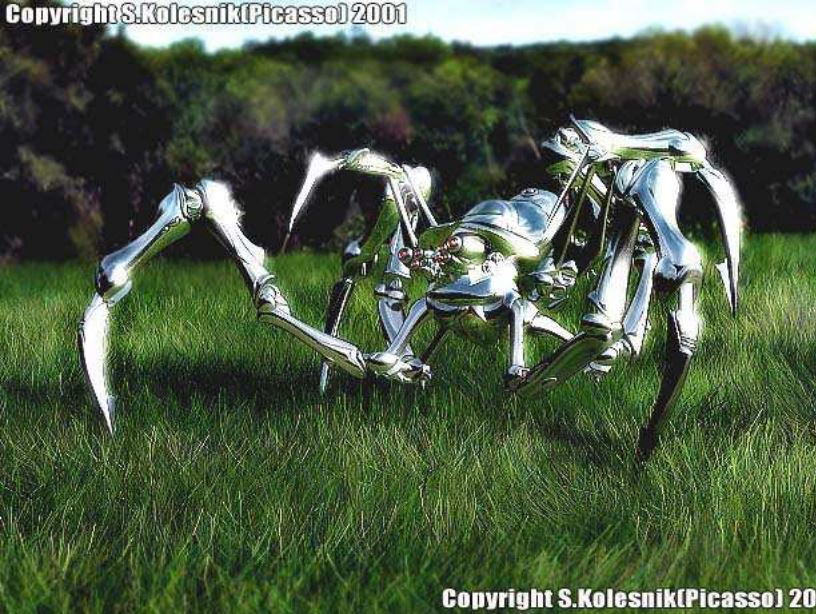
\includegraphics[width=0.75\textwidth]{Cap2/spiderrobot}
\caption{Cupim cibernético.}\label{FDIII}
\end{figure}

Considerando um robô manipulador rígido, malha aberta, e de $n$-juntas em série. Seja $q$ a representação de seu vetor de posição angular das juntas  e $\tau$ a representação de seu vetor de torque. A equação dinâmica pelo método de
Lagrange é dada por:
\begin{equation} \label{eq:lagr1}
\frac{d}{dt} \left( \frac{\partial L}{\partial \dot{q}} \right) -\frac{\partial L}{\partial q}=\tau^{T}.
\end{equation}
O Lagrangiano $L$ é definido como a diferença entre as energias cinética e potencial do sistema:
\begin{equation} \label{L}
L=T-P
\end{equation}

A energia cinética total dos ligamentos é representada:
\begin{equation} \label{energT}
T=\frac{1}{2}\dot{q}^{T}M(q)\dot{q}
\end{equation}


% \chapter{Controle Robusto de Concretos Caóticos}
% \section{Controle combinado}
Conforme vimos na seção \ref{ectq3} podemos controlar um sistema nao linear como  através da técnica do torque computado, usando um controlador PD dado por:
\begin{equation} \label{ectq3}
\tau'=\ddot{q}_d+K_v(\dot{q}_d-\dot{q})+K_p(q_d-q) \; ,
\end{equation}
sendo $q_{d}$, $\dot{q}_{d}$ e $\ddot{q}_{d}$ a posição desejada, a velocidade desejada e a aceleração desejada; $K_p$
e $K_v$ são matrizes diagonais $n \times n$, sendo que cada elemento da diagonal é um ganho positivo e escalar.

Aqui $M_{est}$ e $b_{est}$ são modelos estimados da matriz de inércia, $M$, e do vetor de torques não inerciais, $b$, do robô real,  respectivamente. A equação de malha fechada do sistema é:
\begin{equation} \label{ectq4}
\ddot{e}+K_v\dot{e}+K_pe=M_{est}^{-1}[(M-M_{est})\ddot{q}+(b-b_{est})] \; .
\end{equation}

Em um manipulador real, podem existir distúrbios externos tais como atrito, variação de torque dos atuadores, e perturbações em virtude  das cargas no robô. Se a soma destes distúrbios for definida como $d_{ext}$ e adicionada à (\ref{ectq4}), teremos
\begin{equation} \label{ectq5}
\ddot{e}+K_v\dot{e}+K_pe=M_{est}^{-1}[(M-M_{est})\ddot{q}+(b-b_{est})+d_{ext}] \; .
\end{equation}


% \chapter{Conclusão}
% %\section{Conclusão}

Neste trabalho realizou-se o projeto de uma metodologia de controle subótimo redundante da junta passiva de um manipulador com três graus de liberdade instantaneamente. Para este propósito usou-se nas formulações o vetor gradiente de uma função escalar que estima o acoplamento entre a junta passiva e as ativas desse manipulador. Aqui a redundância
foi usada da melhor maneira possível sem focalizar o efeito global. Portanto, este método deve ser denominado de \emph{controle ótimo local por redundância}. A principal vantagem dessa formulação é a computação em tempo real, que é
necessária para o controle do manipulador experimental. Além disso esse método pode ser usado com diferentes tipos de controladores, uma vez que as alterações são feitas nas equações dinâmicas do manipulador.

A consequência direta observada nessa formulação é a redução dos torques na fase de controle da junta passiva, e consequente redução da energia elétrica gasta. Isso ocorre devido ao fato de que ao longo da trajetória do manipulador
o índice de acoplamento de torque tende a ser maximizado, e portanto, menor é o torque necessário nos atuadores para se conseguir o posicionamento da junta passiva do manipulador.

Outros resultados indiretos obtidos são: um movimento mais uniforme e suave do manipulador e um tempo de acomodação menor tanto no posicionamento da junta passiva quanto das ativas, conforme podemos obervar nos gráficos de desempenho dos resultados apresentados. Isso ocorre porque a maximização do acoplamento entre as juntas facilita o controle. Assim
ocorrem menos picos de torque, e como as juntas ativas tem ``menos trabalho'' para posicionar a passiva estas se movem menos na direçao contrária ao movimento daquelas, diminuindo assim as velocidades alcançadas e os tempos de posicionamento.

Uma extensão deste trabalho pode ser a implementação de um \emph{controle ótimo global por redundância} da junta passiva do manipulador. Para isto pode-se fazer o planejamento \emph{off-line} da trajetória das juntas de modo a minimizar a energia consumida. Alguns estudos foram feitos nesse sentido, usando o Princípio Mínimo de Pontryagin, mas sem resultados satisfatórios até o momento.


% REFERENCIAS BIBLIOGRAFICAS
\renewcommand\bibname{\itareferencesnamebabel} %renomear título do capítulo referências
\printbibliography

% Apendices
\appendix
\chapter{Tópicos de Dilema Linear} %opcional
\section{Uma Primeira Seção para o Apêndice}

A matriz de Dilema Linear $M$ e o vetor de torques inerciais $b$,
utilizados na simulação são calculados segundo a formulação 
abaixo:
\begin{equation}
M=\left[ \begin{array}{ccc}
M_{11} & M_{12} & M_{13} \\
M_{21} & M_{22} & M_{23} \\
M_{31} & M_{32} & M_{33}
\end{array} \right]
\end{equation}

\begin{figure}[h]
\centering
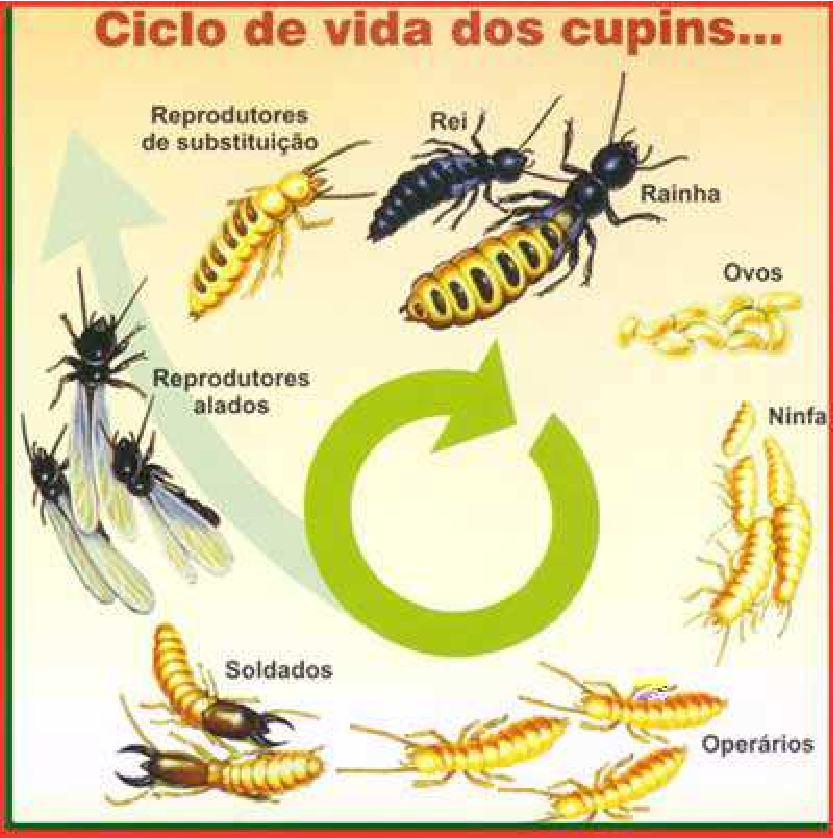
\includegraphics[height=5cm, width=5cm]{ApeA/pragas_ciclo_cupim}
\caption{Uma figura que está no apêndice}\label{FD}
\end{figure}


% Anexos
\annex
\chapter{Exemplo de um Primeiro Anexo} %opcional
% Texto do Primeiro Anexo
\section{Uma Seção do Primeiro Anexo}
% Texto da primeira secao do primeiro anexo
Algum texto na primeira seção do primeiro anexo.



% Glossario
%\itaglossary
%\printglossary

% Folha de Registro do Documento
% Valores dos campos do formulario
\FRDitadata{25 de março de 2015}
\FRDitadocnro{DCTA/ITA/DM-018/2015} %(o número de registro você solicita a biblioteca)
\FRDitaorgaointerno{Instituto Tecnológico de Aeronáutica -- ITA}
%Exemplo no caso de pós-graduação: Instituto Tecnol{\'o}gico de Aeron{\'a}utica -- ITA
\FRDitapalavrasautor{Cupim; Cimento; Estruturas}
\FRDitapalavrasresult{Cupim; Dilema; Construção}
%Exemplo no caso de graduação (TG):
%\FRDitapalavraapresentacao{Trabalho de Graduação, ITA, São José dos Campos, 2015. \NumPenultimaPagina\ páginas.}
%Exemplo no caso de pós-graduação (msc, dsc):
\FRDitapalavraapresentacao{ITA, São José dos Campos. Curso de Mestrado. Programa de Pós-Graduação em Engenharia Aeronáutica e Mecânica. Área de Sistemas Aeroespaciais e Mecatrônica. Orientador: Prof.~Dr. Adalberto Santos Dupont. Coorientadora: Prof$^\textnormal{a}$.~Dr$^\textnormal{a}$. Doralice Serra. Defesa em 05/03/2015. Publicada em 25/03/2015.}
\FRDitaresumo{Este trabalho apresenta o processo de desenvolvimento e caracterização de um sistema de vetorização de empuxo com motor a gás frio. O motor tem como requisito empuxo de \(2\;\mathrm{N}\) e \(5\;\mathrm{bar}\) de pressão de câmara. O método de vetorização escolhido para teste foi o de \textit{jet vane}. O motor construído apresentou divergências pequenas com os requisitos, tendo um impulso específico de \(46,6\;\mathrm{s}\). Este motor foi montado em um mecanismo de controle da lâmina defletora e esta montagem foi acoplada a uma balança de três componentes para caracterização das forças e momentos gerados. Como resultado final, obtiveram-se as derivadas de controle de força lateral e momento. Por fim, apresentaram-se os problemas metodológicos encontrados e \textit{trade-offs} de engenharia identificados para o sistema.}
%  Primeiro Parametro: Nacional ou Internacional -- N/I
%  Segundo parametro: Ostensivo, Reservado, Confidencial ou Secreto -- O/R/C/S
\FRDitaOpcoes{N}{O}
% Cria o formulario
\itaFRD

\end{document}
% Fim do Documento. O massacre acabou!!! :-)
